% Options for packages loaded elsewhere
\PassOptionsToPackage{unicode}{hyperref}
\PassOptionsToPackage{hyphens}{url}
%
\documentclass[
]{article}
\usepackage{lmodern}
\usepackage{amssymb,amsmath}
\usepackage{ifxetex,ifluatex}
\ifnum 0\ifxetex 1\fi\ifluatex 1\fi=0 % if pdftex
  \usepackage[T1]{fontenc}
  \usepackage[utf8]{inputenc}
  \usepackage{textcomp} % provide euro and other symbols
\else % if luatex or xetex
  \usepackage{unicode-math}
  \defaultfontfeatures{Scale=MatchLowercase}
  \defaultfontfeatures[\rmfamily]{Ligatures=TeX,Scale=1}
\fi
% Use upquote if available, for straight quotes in verbatim environments
\IfFileExists{upquote.sty}{\usepackage{upquote}}{}
\IfFileExists{microtype.sty}{% use microtype if available
  \usepackage[]{microtype}
  \UseMicrotypeSet[protrusion]{basicmath} % disable protrusion for tt fonts
}{}
\makeatletter
\@ifundefined{KOMAClassName}{% if non-KOMA class
  \IfFileExists{parskip.sty}{%
    \usepackage{parskip}
  }{% else
    \setlength{\parindent}{0pt}
    \setlength{\parskip}{6pt plus 2pt minus 1pt}}
}{% if KOMA class
  \KOMAoptions{parskip=half}}
\makeatother
\usepackage{xcolor}
\IfFileExists{xurl.sty}{\usepackage{xurl}}{} % add URL line breaks if available
\IfFileExists{bookmark.sty}{\usepackage{bookmark}}{\usepackage{hyperref}}
\hypersetup{
  pdftitle={A report generated from a pure R script},
  hidelinks,
  pdfcreator={LaTeX via pandoc}}
\urlstyle{same} % disable monospaced font for URLs
\usepackage[margin=1in]{geometry}
\usepackage{color}
\usepackage{fancyvrb}
\newcommand{\VerbBar}{|}
\newcommand{\VERB}{\Verb[commandchars=\\\{\}]}
\DefineVerbatimEnvironment{Highlighting}{Verbatim}{commandchars=\\\{\}}
% Add ',fontsize=\small' for more characters per line
\usepackage{framed}
\definecolor{shadecolor}{RGB}{248,248,248}
\newenvironment{Shaded}{\begin{snugshade}}{\end{snugshade}}
\newcommand{\AlertTok}[1]{\textcolor[rgb]{0.94,0.16,0.16}{#1}}
\newcommand{\AnnotationTok}[1]{\textcolor[rgb]{0.56,0.35,0.01}{\textbf{\textit{#1}}}}
\newcommand{\AttributeTok}[1]{\textcolor[rgb]{0.77,0.63,0.00}{#1}}
\newcommand{\BaseNTok}[1]{\textcolor[rgb]{0.00,0.00,0.81}{#1}}
\newcommand{\BuiltInTok}[1]{#1}
\newcommand{\CharTok}[1]{\textcolor[rgb]{0.31,0.60,0.02}{#1}}
\newcommand{\CommentTok}[1]{\textcolor[rgb]{0.56,0.35,0.01}{\textit{#1}}}
\newcommand{\CommentVarTok}[1]{\textcolor[rgb]{0.56,0.35,0.01}{\textbf{\textit{#1}}}}
\newcommand{\ConstantTok}[1]{\textcolor[rgb]{0.00,0.00,0.00}{#1}}
\newcommand{\ControlFlowTok}[1]{\textcolor[rgb]{0.13,0.29,0.53}{\textbf{#1}}}
\newcommand{\DataTypeTok}[1]{\textcolor[rgb]{0.13,0.29,0.53}{#1}}
\newcommand{\DecValTok}[1]{\textcolor[rgb]{0.00,0.00,0.81}{#1}}
\newcommand{\DocumentationTok}[1]{\textcolor[rgb]{0.56,0.35,0.01}{\textbf{\textit{#1}}}}
\newcommand{\ErrorTok}[1]{\textcolor[rgb]{0.64,0.00,0.00}{\textbf{#1}}}
\newcommand{\ExtensionTok}[1]{#1}
\newcommand{\FloatTok}[1]{\textcolor[rgb]{0.00,0.00,0.81}{#1}}
\newcommand{\FunctionTok}[1]{\textcolor[rgb]{0.00,0.00,0.00}{#1}}
\newcommand{\ImportTok}[1]{#1}
\newcommand{\InformationTok}[1]{\textcolor[rgb]{0.56,0.35,0.01}{\textbf{\textit{#1}}}}
\newcommand{\KeywordTok}[1]{\textcolor[rgb]{0.13,0.29,0.53}{\textbf{#1}}}
\newcommand{\NormalTok}[1]{#1}
\newcommand{\OperatorTok}[1]{\textcolor[rgb]{0.81,0.36,0.00}{\textbf{#1}}}
\newcommand{\OtherTok}[1]{\textcolor[rgb]{0.56,0.35,0.01}{#1}}
\newcommand{\PreprocessorTok}[1]{\textcolor[rgb]{0.56,0.35,0.01}{\textit{#1}}}
\newcommand{\RegionMarkerTok}[1]{#1}
\newcommand{\SpecialCharTok}[1]{\textcolor[rgb]{0.00,0.00,0.00}{#1}}
\newcommand{\SpecialStringTok}[1]{\textcolor[rgb]{0.31,0.60,0.02}{#1}}
\newcommand{\StringTok}[1]{\textcolor[rgb]{0.31,0.60,0.02}{#1}}
\newcommand{\VariableTok}[1]{\textcolor[rgb]{0.00,0.00,0.00}{#1}}
\newcommand{\VerbatimStringTok}[1]{\textcolor[rgb]{0.31,0.60,0.02}{#1}}
\newcommand{\WarningTok}[1]{\textcolor[rgb]{0.56,0.35,0.01}{\textbf{\textit{#1}}}}
\usepackage{longtable,booktabs}
% Correct order of tables after \paragraph or \subparagraph
\usepackage{etoolbox}
\makeatletter
\patchcmd\longtable{\par}{\if@noskipsec\mbox{}\fi\par}{}{}
\makeatother
% Allow footnotes in longtable head/foot
\IfFileExists{footnotehyper.sty}{\usepackage{footnotehyper}}{\usepackage{footnote}}
\makesavenoteenv{longtable}
\usepackage{graphicx}
\makeatletter
\def\maxwidth{\ifdim\Gin@nat@width>\linewidth\linewidth\else\Gin@nat@width\fi}
\def\maxheight{\ifdim\Gin@nat@height>\textheight\textheight\else\Gin@nat@height\fi}
\makeatother
% Scale images if necessary, so that they will not overflow the page
% margins by default, and it is still possible to overwrite the defaults
% using explicit options in \includegraphics[width, height, ...]{}
\setkeys{Gin}{width=\maxwidth,height=\maxheight,keepaspectratio}
% Set default figure placement to htbp
\makeatletter
\def\fps@figure{htbp}
\makeatother
\setlength{\emergencystretch}{3em} % prevent overfull lines
\providecommand{\tightlist}{%
  \setlength{\itemsep}{0pt}\setlength{\parskip}{0pt}}
\setcounter{secnumdepth}{-\maxdimen} % remove section numbering

\title{A report generated from a pure R script}
\author{}
\date{\vspace{-2.5em}}

\begin{document}
\maketitle

Load the data, plot the data!

\begin{Shaded}
\begin{Highlighting}[]
\KeywordTok{library}\NormalTok{(gridExtra)}
\KeywordTok{library}\NormalTok{(tidymodels)}
\end{Highlighting}
\end{Shaded}

\begin{verbatim}
-- Attaching packages -------------------------------------- tidymodels 0.1.1 --
\end{verbatim}

\begin{verbatim}
v broom     0.7.1      v recipes   0.1.13
v dials     0.0.9      v rsample   0.0.8 
v dplyr     1.0.2      v tibble    3.0.4 
v ggplot2   3.3.2      v tidyr     1.1.2 
v infer     0.5.3      v tune      0.1.1 
v modeldata 0.0.2      v workflows 0.2.1 
v parsnip   0.1.3      v yardstick 0.0.7 
v purrr     0.3.4      
\end{verbatim}

\begin{verbatim}
-- Conflicts ----------------------------------------- tidymodels_conflicts() --
x dplyr::combine() masks gridExtra::combine()
x purrr::discard() masks scales::discard()
x dplyr::filter()  masks stats::filter()
x dplyr::lag()     masks stats::lag()
x recipes::step()  masks stats::step()
\end{verbatim}

\begin{Shaded}
\begin{Highlighting}[]
\KeywordTok{library}\NormalTok{(lubridate)}
\end{Highlighting}
\end{Shaded}

\begin{verbatim}
Attaching package: 'lubridate'
\end{verbatim}

\begin{verbatim}
The following objects are masked from 'package:base':

    date, intersect, setdiff, union
\end{verbatim}

\begin{Shaded}
\begin{Highlighting}[]
\KeywordTok{library}\NormalTok{(readxl)}
\KeywordTok{library}\NormalTok{(ggcorrplot)}
\KeywordTok{library}\NormalTok{(knitr)}
\KeywordTok{library}\NormalTok{(rpart.plot)}
\end{Highlighting}
\end{Shaded}

\begin{verbatim}
Loading required package: rpart
\end{verbatim}

\begin{verbatim}
Attaching package: 'rpart'
\end{verbatim}

\begin{verbatim}
The following object is masked from 'package:dials':

    prune
\end{verbatim}

\begin{Shaded}
\begin{Highlighting}[]
\KeywordTok{library}\NormalTok{(randomForestExplainer)}
\end{Highlighting}
\end{Shaded}

\begin{verbatim}
Registered S3 method overwritten by 'GGally':
  method from   
  +.gg   ggplot2
\end{verbatim}

\begin{Shaded}
\begin{Highlighting}[]
\KeywordTok{library}\NormalTok{(doParallel)}
\end{Highlighting}
\end{Shaded}

\begin{verbatim}
Loading required package: foreach
\end{verbatim}

\begin{verbatim}
Attaching package: 'foreach'
\end{verbatim}

\begin{verbatim}
The following objects are masked from 'package:purrr':

    accumulate, when
\end{verbatim}

\begin{verbatim}
Loading required package: iterators
\end{verbatim}

\begin{verbatim}
Loading required package: parallel
\end{verbatim}

\begin{Shaded}
\begin{Highlighting}[]
\KeywordTok{library}\NormalTok{(vip)}
\end{Highlighting}
\end{Shaded}

\begin{verbatim}
Attaching package: 'vip'
\end{verbatim}

\begin{verbatim}
The following object is masked from 'package:utils':

    vi
\end{verbatim}

\begin{Shaded}
\begin{Highlighting}[]
\KeywordTok{require}\NormalTok{(ggplot2)}
\KeywordTok{require}\NormalTok{(dplyr)}
\KeywordTok{require}\NormalTok{(ggcorrplot)}
\KeywordTok{require}\NormalTok{(broom)}


\NormalTok{data.dir <{-}}\StringTok{ "./data/"}
\NormalTok{petrale <{-}}\StringTok{ }\KeywordTok{read.csv}\NormalTok{(}\KeywordTok{file.path}\NormalTok{(data.dir,}\StringTok{"Petrale\_analyzed.data.csv"}\NormalTok{))}
\NormalTok{sable <{-}}\StringTok{ }\KeywordTok{read.csv}\NormalTok{(}\KeywordTok{file.path}\NormalTok{(data.dir,}\StringTok{"Sablefish\_Analyzed\_Data\_north.csv"}\NormalTok{))}
\NormalTok{sable\_DFA <{-}}\StringTok{ }\KeywordTok{read.csv}\NormalTok{(}\KeywordTok{file.path}\NormalTok{(data.dir,}\StringTok{"Sablefish\_DFA\_Data.csv"}\NormalTok{))}

\KeywordTok{names}\NormalTok{(petrale)}
\end{Highlighting}
\end{Shaded}

\begin{verbatim}
 [1] "year"       "X"          "total.bio"  "sp.bio"     "depletion" 
 [6] "age.0"      "spr"        "expl.rate"  "sp.bio.sd"  "age.0.sd"  
[11] "yrminusone" "resids"     "log.resids" "SR_pred"    "Label"     
[16] "dev"        "devsd"      "DDpre"      "Tpre.a"     "Tpre.b"    
[21] "MLDegg"     "LSTegg"     "CSTegg1"    "DDegg1"     "CSTegg2"   
[26] "LSTegg2"    "DDegg2"     "LSTlarv"    "CSTlarv"    "DDlarv"    
[31] "LSTpjuv"    "CSTpjuv"    "DDpjuv"     "LSTbjuv.a"  "CSTbjuv.a" 
[36] "LSTbjuv.b"  "CSTbjuv.b" 
\end{verbatim}

\begin{Shaded}
\begin{Highlighting}[]
\CommentTok{\#Plot recruits vs year and spawning stock biomass}
\KeywordTok{plot}\NormalTok{(age}\FloatTok{.0}\OperatorTok{\textasciitilde{}}\NormalTok{year,}\DataTypeTok{data=}\NormalTok{petrale, }\DataTypeTok{type=}\StringTok{"l"}\NormalTok{, }\DataTypeTok{main=}\StringTok{"Recruits per year"}\NormalTok{)}
\end{Highlighting}
\end{Shaded}

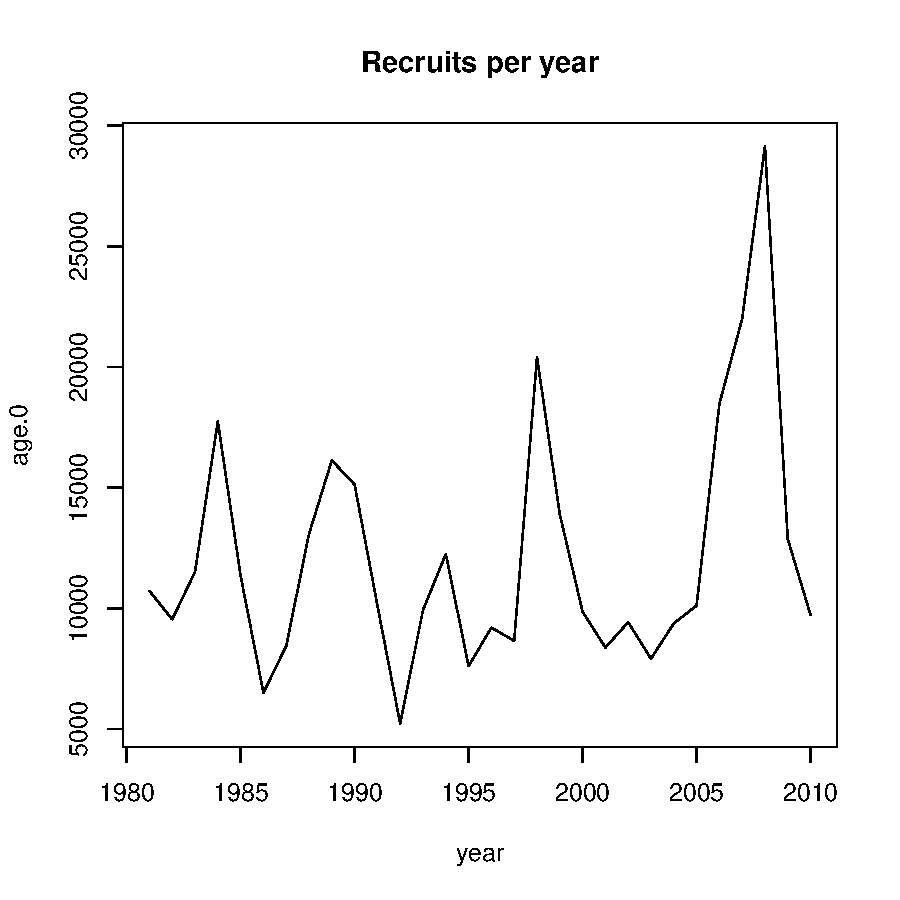
\includegraphics{calcurr_files/figure-latex/unnamed-chunk-1-1.pdf}

\begin{Shaded}
\begin{Highlighting}[]
\KeywordTok{plot}\NormalTok{(age}\FloatTok{.0}\OperatorTok{\textasciitilde{}}\NormalTok{sp.bio,}\DataTypeTok{data=}\NormalTok{petrale, }\DataTypeTok{main=}\StringTok{"Recruits vs SSB"}\NormalTok{)}
\end{Highlighting}
\end{Shaded}

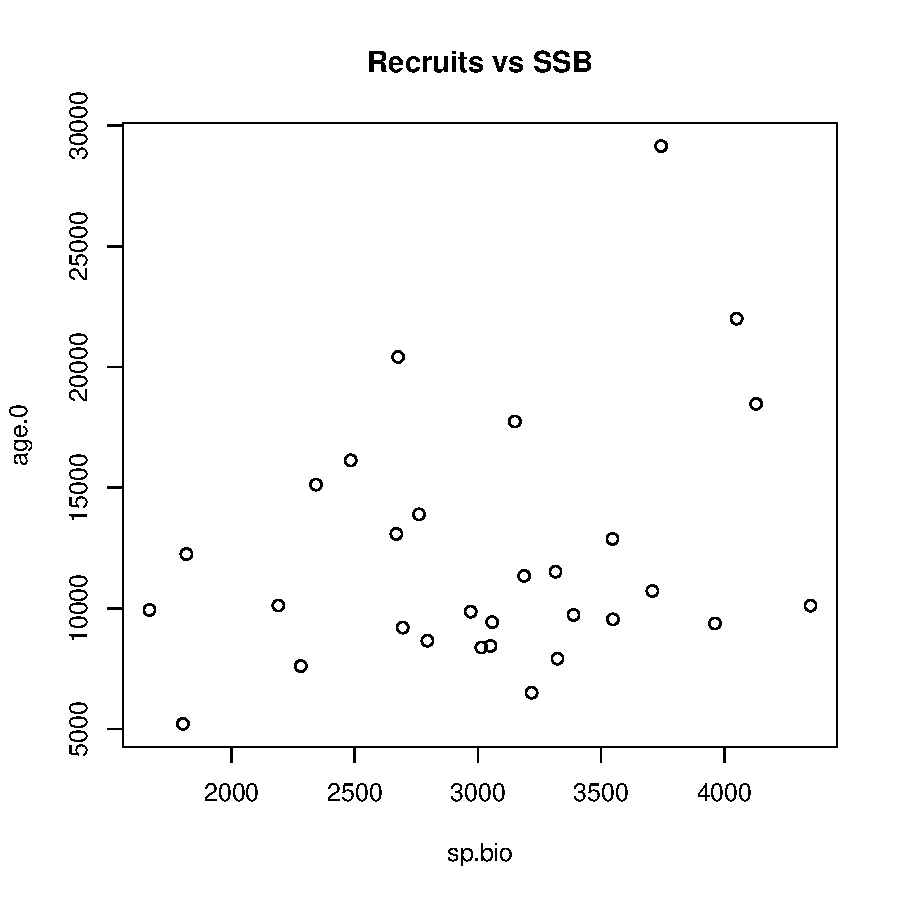
\includegraphics{calcurr_files/figure-latex/unnamed-chunk-1-2.pdf}

Spawning biomass and recruitment are not very correlated..not
surprising.

\begin{Shaded}
\begin{Highlighting}[]
\CommentTok{\#Plot correlation}
\KeywordTok{round}\NormalTok{(}\KeywordTok{cor}\NormalTok{(petrale }\OperatorTok{\%>\%}\StringTok{ }
\StringTok{            }\NormalTok{dplyr}\OperatorTok{::}\KeywordTok{select}\NormalTok{(}\KeywordTok{names}\NormalTok{(petrale)[}\DecValTok{18}\OperatorTok{:}\DecValTok{37}\NormalTok{]) }\OperatorTok{\%>\%}\StringTok{ }\NormalTok{data.frame), }\DecValTok{1}\NormalTok{) }\OperatorTok{\%>\%}\StringTok{ }
\KeywordTok{ggcorrplot}\NormalTok{(}\DataTypeTok{tl.cex=}\DecValTok{6}\NormalTok{)}
\end{Highlighting}
\end{Shaded}

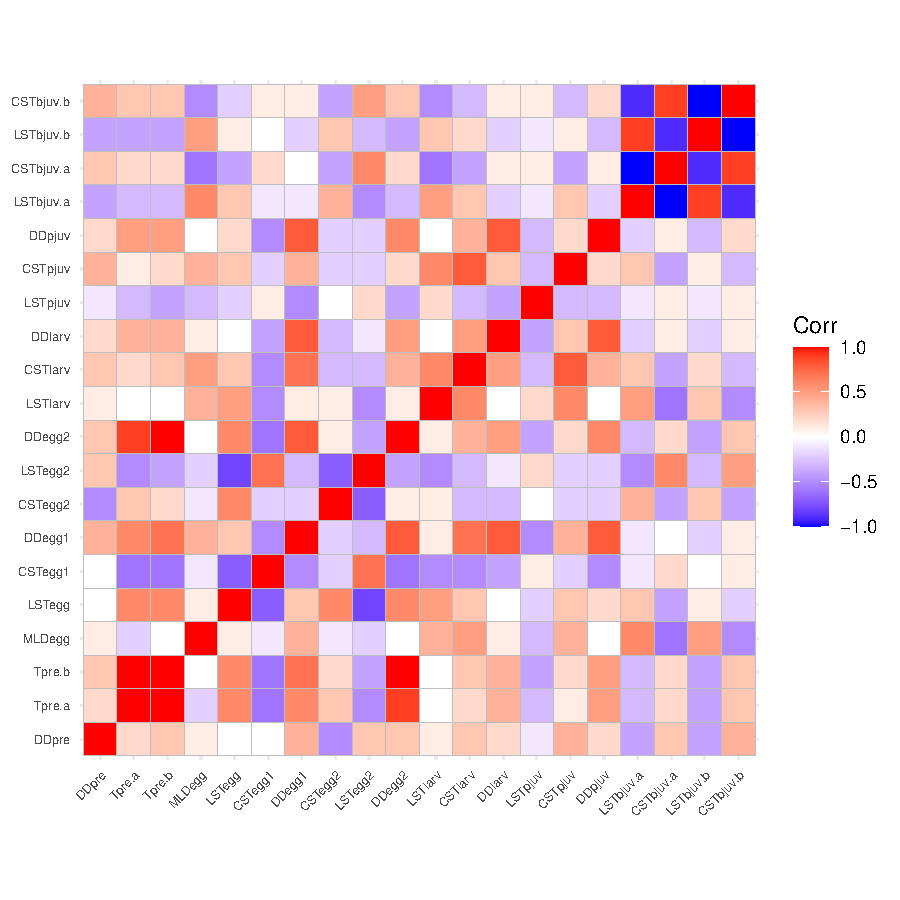
\includegraphics{calcurr_files/figure-latex/unnamed-chunk-2-1.pdf}

\begin{Shaded}
\begin{Highlighting}[]
\NormalTok{modpetrale <{-}}\StringTok{ }\NormalTok{petrale }\OperatorTok{\%>\%}
\StringTok{  }\KeywordTok{select}\NormalTok{(}\OperatorTok{{-}}\KeywordTok{c}\NormalTok{(X,total.bio,depletion,spr,expl.rate,sp.bio.sd,age.}\FloatTok{0.}\NormalTok{sd,yrminusone,resids,log.resids,SR\_pred,Label,dev,devsd, LSTbjuv.a,CSTbjuv.a,CSTbjuv.b, Tpre.b, DDegg2)) }\OperatorTok{\%>\%}
\StringTok{  }\KeywordTok{pivot\_longer}\NormalTok{(}
    \DataTypeTok{cols=}\OperatorTok{{-}}\KeywordTok{c}\NormalTok{(year,sp.bio,age}\FloatTok{.0}\NormalTok{),}
    \DataTypeTok{values\_to=}\StringTok{"covs\_val"}\NormalTok{)}
\end{Highlighting}
\end{Shaded}

The time series for LST \& CST are highly correlated, also Tpre.a and
Tpre.b and DDegg and DDegg2. I remove correlated predictors below

\begin{Shaded}
\begin{Highlighting}[]
\CommentTok{\#Do regression with different environmental time series}
\NormalTok{modpetrale }\OperatorTok{\%>\%}\StringTok{ }
\StringTok{  }\KeywordTok{group\_by}\NormalTok{(name) }\OperatorTok{\%>\%}
\StringTok{  }\KeywordTok{do}\NormalTok{(}\KeywordTok{glance}\NormalTok{(}\KeywordTok{lm}\NormalTok{(age}\FloatTok{.0}\OperatorTok{\textasciitilde{}}\NormalTok{sp.bio}\OperatorTok{+}\NormalTok{covs\_val,}\DataTypeTok{data=}\NormalTok{.))) }\OperatorTok{\%>\%}
\StringTok{  }\KeywordTok{bind\_rows}\NormalTok{(modpetrale }\OperatorTok{\%>\%}\StringTok{ }
\StringTok{              }\NormalTok{dplyr}\OperatorTok{::}\KeywordTok{select}\NormalTok{(}\OperatorTok{{-}}\KeywordTok{c}\NormalTok{(covs\_val,name)) }\OperatorTok{\%>\%}
\StringTok{              }\KeywordTok{distinct}\NormalTok{() }\OperatorTok{\%>\%}\StringTok{ }
\StringTok{              }\KeywordTok{do}\NormalTok{(}\KeywordTok{glance}\NormalTok{(}\KeywordTok{lm}\NormalTok{(age}\FloatTok{.0}\OperatorTok{\textasciitilde{}}\NormalTok{sp.bio,}\DataTypeTok{data=}\NormalTok{.))) }\OperatorTok{\%>\%}
\StringTok{              }\KeywordTok{mutate}\NormalTok{(}\DataTypeTok{name=}\StringTok{"sp.bio only"}\NormalTok{)) }\OperatorTok{\%>\%}
\StringTok{  }\KeywordTok{arrange}\NormalTok{(}\OperatorTok{{-}}\NormalTok{adj.r.squared) }\OperatorTok{\%>\%}\StringTok{ }
\StringTok{  }\KeywordTok{mutate}\NormalTok{(}\KeywordTok{across}\NormalTok{(}\KeywordTok{where}\NormalTok{(is.double), round, }\DecValTok{3}\NormalTok{)) }\OperatorTok{\%>\%}\StringTok{ }
\StringTok{  }\NormalTok{dplyr}\OperatorTok{::}\KeywordTok{select}\NormalTok{(}\OperatorTok{{-}}\KeywordTok{c}\NormalTok{(r.squared,logLik)) }\OperatorTok{\%>\%}\StringTok{ }
\StringTok{  }\NormalTok{data.frame }\OperatorTok{\%>\%}
\StringTok{  }\KeywordTok{kable}\NormalTok{()}
\end{Highlighting}
\end{Shaded}

\begin{longtable}[]{@{}lrrrrrrrrrr@{}}
\toprule
name & adj.r.squared & sigma & statistic & p.value & df & AIC & BIC &
deviance & df.residual & nobs\tabularnewline
\midrule
\endhead
MLDegg & 0.220 & 4554.594 & 5.087 & 0.013 & 2 & 595.409 & 601.014 &
560096709 & 27 & 30\tabularnewline
DDpre & 0.191 & 4638.122 & 4.423 & 0.022 & 2 & 596.499 & 602.104 &
580828684 & 27 & 30\tabularnewline
LSTbjuv.b & 0.110 & 4865.588 & 2.787 & 0.079 & 2 & 599.372 & 604.977 &
639196568 & 27 & 30\tabularnewline
CSTegg1 & 0.106 & 4875.859 & 2.718 & 0.084 & 2 & 599.499 & 605.103 &
641897960 & 27 & 30\tabularnewline
DDpjuv & 0.073 & 4964.367 & 2.145 & 0.137 & 2 & 600.578 & 606.183 &
665413350 & 27 & 30\tabularnewline
DDlarv & 0.063 & 4990.496 & 1.982 & 0.157 & 2 & 600.893 & 606.498 &
672436272 & 27 & 30\tabularnewline
sp.bio only & 0.047 & 5033.235 & 2.440 & 0.130 & 1 & 600.496 & 604.699 &
709336806 & 28 & 30\tabularnewline
LSTegg2 & 0.038 & 5058.523 & 1.568 & 0.227 & 2 & 601.705 & 607.310 &
690893677 & 27 & 30\tabularnewline
Tpre.a & 0.024 & 5095.462 & 1.350 & 0.276 & 2 & 602.142 & 607.747 &
701020668 & 27 & 30\tabularnewline
LSTegg & 0.022 & 5099.084 & 1.329 & 0.281 & 2 & 602.184 & 607.789 &
702017715 & 27 & 30\tabularnewline
CSTlarv & 0.021 & 5101.732 & 1.314 & 0.285 & 2 & 602.216 & 607.820 &
702747084 & 27 & 30\tabularnewline
CSTpjuv & 0.014 & 5121.648 & 1.199 & 0.317 & 2 & 602.449 & 608.054 &
708244423 & 27 & 30\tabularnewline
CSTegg2 & 0.013 & 5124.069 & 1.185 & 0.321 & 2 & 602.478 & 608.083 &
708914144 & 27 & 30\tabularnewline
DDegg1 & 0.012 & 5124.367 & 1.183 & 0.322 & 2 & 602.481 & 608.086 &
708996791 & 27 & 30\tabularnewline
LSTpjuv & 0.012 & 5125.006 & 1.180 & 0.323 & 2 & 602.489 & 608.094 &
709173555 & 27 & 30\tabularnewline
LSTlarv & 0.012 & 5125.596 & 1.176 & 0.324 & 2 & 602.496 & 608.100 &
709336801 & 27 & 30\tabularnewline
\bottomrule
\end{longtable}

The best covariates are MLDegg (Mean mixed layer depth) and spawner
preconditioning degree-days, none other \textless.05

\begin{Shaded}
\begin{Highlighting}[]
\NormalTok{wide\_petrale <{-}}\StringTok{ }\NormalTok{modpetrale }\OperatorTok{\%>\%}
\StringTok{  }\KeywordTok{pivot\_wider}\NormalTok{(}\DataTypeTok{names\_from =}\NormalTok{ name, }\DataTypeTok{values\_from=}\NormalTok{covs\_val) }\OperatorTok{\%>\%}
\StringTok{  }\KeywordTok{select}\NormalTok{(}\OperatorTok{{-}}\KeywordTok{c}\NormalTok{(year))}

\KeywordTok{set.seed}\NormalTok{(}\DecValTok{100}\NormalTok{)}
\NormalTok{pet\_split <{-}}\StringTok{ }\KeywordTok{initial\_split}\NormalTok{(wide\_petrale) }\CommentTok{\#By default, 3/4 data going into training; 1/4 test}
\NormalTok{pet\_train <{-}}\StringTok{ }\KeywordTok{training}\NormalTok{(pet\_split)}
\NormalTok{pet\_test <{-}}\StringTok{ }\KeywordTok{testing}\NormalTok{(pet\_split)}

\NormalTok{pet\_split }\CommentTok{\# View the pet\_split object.}
\end{Highlighting}
\end{Shaded}

\begin{verbatim}
<Analysis/Assess/Total>
<23/7/30>
\end{verbatim}

\begin{Shaded}
\begin{Highlighting}[]
\CommentTok{\#Package not working for now, fix later}
\KeywordTok{source}\NormalTok{(}\StringTok{"R/fit\_split.R"}\NormalTok{)}

\NormalTok{lm\_spec <{-}}\StringTok{ }\KeywordTok{linear\_reg}\NormalTok{() }\OperatorTok{\%>\%}\StringTok{ }
\StringTok{  }\KeywordTok{set\_engine}\NormalTok{(}\StringTok{"lm"}\NormalTok{)}

\CommentTok{\#  Use the workflows and tidymodels function from above to fit a model to the training data}
\NormalTok{lm\_fit <{-}}\StringTok{ }\KeywordTok{fit\_split}\NormalTok{(age}\FloatTok{.0}\OperatorTok{\textasciitilde{}}\NormalTok{sp.bio}\OperatorTok{+}\NormalTok{MLDegg, }\CommentTok{\# specify formula}
                    \DataTypeTok{model=}\NormalTok{lm\_spec, }\CommentTok{\# specify model}
                    \DataTypeTok{split=}\NormalTok{pet\_split) }\CommentTok{\# specify data}

\NormalTok{lm\_fit }\OperatorTok{\%>\%}\StringTok{ }
\StringTok{  }\KeywordTok{collect\_metrics}\NormalTok{()}
\end{Highlighting}
\end{Shaded}

\begin{verbatim}
# A tibble: 2 x 3
  .metric .estimator .estimate
  <chr>   <chr>          <dbl>
1 rmse    standard   4434.    
2 rsq     standard      0.0534
\end{verbatim}

\begin{Shaded}
\begin{Highlighting}[]
\NormalTok{lm\_fit }\OperatorTok{\%>\%}
\StringTok{  }\KeywordTok{collect\_predictions}\NormalTok{()}
\end{Highlighting}
\end{Shaded}

\begin{verbatim}
# A tibble: 7 x 4
  id                .pred  .row age.0
  <chr>             <dbl> <int> <int>
1 train/test split 11066.     6  6509
2 train/test split  9283.    10 15129
3 train/test split  9801.    14 12252
4 train/test split 10428.    16  9207
5 train/test split 14158.    19 13899
6 train/test split 14484.    23  7919
7 train/test split 15778.    25 10118
\end{verbatim}

\begin{Shaded}
\begin{Highlighting}[]
\NormalTok{lm\_fit }\OperatorTok{\%>\%}\StringTok{ }
\StringTok{  }\NormalTok{collect\_predictions }\OperatorTok{\%>\%}\StringTok{ }\CommentTok{\# from tune package, predicting using test data}
\StringTok{  }\KeywordTok{mutate}\NormalTok{(}\DataTypeTok{resid=}\NormalTok{(age}\FloatTok{.0}\OperatorTok{{-}}\NormalTok{.pred)}\OperatorTok{\^{}}\DecValTok{2}\NormalTok{) }\OperatorTok{\%>\%}\StringTok{ }\CommentTok{\#calculate squared residuals}
\StringTok{  }\KeywordTok{summarise}\NormalTok{(}\DataTypeTok{rmse=}\KeywordTok{sqrt}\NormalTok{(}\KeywordTok{mean}\NormalTok{(resid)))}
\end{Highlighting}
\end{Shaded}

\begin{verbatim}
# A tibble: 1 x 1
   rmse
  <dbl>
1 4434.
\end{verbatim}

\begin{Shaded}
\begin{Highlighting}[]
\KeywordTok{fit\_split}\NormalTok{(age}\FloatTok{.0}\OperatorTok{\textasciitilde{}}\NormalTok{sp.bio}\OperatorTok{+}\NormalTok{MLDegg, }\CommentTok{\# specify formula}
          \DataTypeTok{model=}\NormalTok{lm\_spec, }\CommentTok{\# specify model}
          \DataTypeTok{metrics=}\KeywordTok{metric\_set}\NormalTok{(rmse,mae,mape), }\CommentTok{\#specify model evaluation criteria.}
          \DataTypeTok{split=}\NormalTok{pet\_split) }\OperatorTok{\%>\%}\StringTok{ }
\StringTok{  }\KeywordTok{collect\_metrics}\NormalTok{()}
\end{Highlighting}
\end{Shaded}

\begin{verbatim}
# A tibble: 3 x 3
  .metric .estimator .estimate
  <chr>   <chr>          <dbl>
1 rmse    standard      4434. 
2 mae     standard      3794. 
3 mape    standard        40.4
\end{verbatim}

\begin{Shaded}
\begin{Highlighting}[]
\CommentTok{\#Create new split}
\KeywordTok{set.seed}\NormalTok{(}\DecValTok{100}\NormalTok{)}
\NormalTok{pet\_split <{-}}\StringTok{ }\KeywordTok{initial\_split}\NormalTok{(wide\_petrale)}
\NormalTok{pet\_train <{-}}\StringTok{ }\KeywordTok{training}\NormalTok{(pet\_split)}
\NormalTok{pet\_test <{-}}\StringTok{ }\KeywordTok{testing}\NormalTok{(pet\_split)}

\CommentTok{\#Look at range of data to see if we need to center/scale}
\KeywordTok{apply}\NormalTok{(wide\_petrale,}\DecValTok{2}\NormalTok{,range)}
\end{Highlighting}
\end{Shaded}

\begin{verbatim}
     sp.bio age.0   DDpre   Tpre.a   MLDegg      LSTegg      CSTegg1  DDegg1
[1,]   1667  5219 173.220 5.712132 31.04178 -0.04620180 -0.003487927 204.601
[2,]   4350 29151 255.921 6.723658 55.73978  0.07280556  0.002003658 303.633
         CSTegg2      LSTegg2     LSTlarv      CSTlarv  DDlarv     LSTpjuv
[1,] -0.01636910 -0.001686707 -0.04468344 -0.003200462 270.312 -0.06701870
[2,]  0.02833067  0.000878600  0.04510549  0.020146587 388.420  0.04350774
         CSTpjuv  DDpjuv   LSTbjuv.b
[1,] -0.00782200 157.945 0.001798998
[2,]  0.01081297 219.048 0.047165717
\end{verbatim}

\begin{Shaded}
\begin{Highlighting}[]
\CommentTok{\#  Create a recipe.}
\NormalTok{pet\_recipe <{-}}\StringTok{ }\KeywordTok{recipe}\NormalTok{(age}\FloatTok{.0}\OperatorTok{\textasciitilde{}}\NormalTok{.,}\DataTypeTok{data=}\NormalTok{pet\_train) }\OperatorTok{\%>\%}\StringTok{ }
\StringTok{  }\KeywordTok{step\_center}\NormalTok{(MLDegg) }\OperatorTok{\%>\%}\StringTok{ }
\StringTok{  }\KeywordTok{step\_scale}\NormalTok{(MLDegg) }

\CommentTok{\#  Prep the recipe. }
\NormalTok{pet\_prep <{-}}\StringTok{ }\NormalTok{pet\_recipe }\OperatorTok{\%>\%}\StringTok{ }
\StringTok{  }\KeywordTok{prep}\NormalTok{(}\DataTypeTok{training=}\NormalTok{pet\_train,}\DataTypeTok{retain=}\OtherTok{TRUE}\NormalTok{)}

\NormalTok{pet\_prep}
\end{Highlighting}
\end{Shaded}

\begin{verbatim}
Data Recipe

Inputs:

      role #variables
   outcome          1
 predictor         16

Training data contained 23 data points and no missing data.

Operations:

Centering for MLDegg [trained]
Scaling for MLDegg [trained]
\end{verbatim}

\begin{Shaded}
\begin{Highlighting}[]
\NormalTok{dt\_model <{-}}\StringTok{ }\KeywordTok{decision\_tree}\NormalTok{(}\DataTypeTok{min\_n=}\DecValTok{5}\NormalTok{,}\DataTypeTok{tree\_depth=}\DecValTok{10}\NormalTok{) }\OperatorTok{\%>\%}\StringTok{ }
\StringTok{  }\KeywordTok{set\_engine}\NormalTok{(}\StringTok{"rpart"}\NormalTok{) }\OperatorTok{\%>\%}\StringTok{  }\CommentTok{\# Specify the R library}
\StringTok{  }\KeywordTok{set\_mode}\NormalTok{(}\StringTok{"regression"}\NormalTok{) }\OperatorTok{\%>\%}\StringTok{  }\CommentTok{\# Specify regression or classification}
\StringTok{  }\KeywordTok{fit}\NormalTok{(age}\FloatTok{.0}\OperatorTok{\textasciitilde{}}\NormalTok{.,}\DataTypeTok{data=}\KeywordTok{juice}\NormalTok{(pet\_prep))}

\NormalTok{rpart.plot}\OperatorTok{::}\KeywordTok{rpart.plot}\NormalTok{(dt\_model}\OperatorTok{$}\NormalTok{fit,}
                       \DataTypeTok{type=}\DecValTok{4}\NormalTok{,}
                       \DataTypeTok{extra=}\DecValTok{101}\NormalTok{,}
                       \DataTypeTok{branch.lty=}\DecValTok{3}\NormalTok{,}
                       \DataTypeTok{nn=}\OtherTok{TRUE}\NormalTok{,}
                       \DataTypeTok{roundint=}\OtherTok{FALSE}\NormalTok{) }
\end{Highlighting}
\end{Shaded}

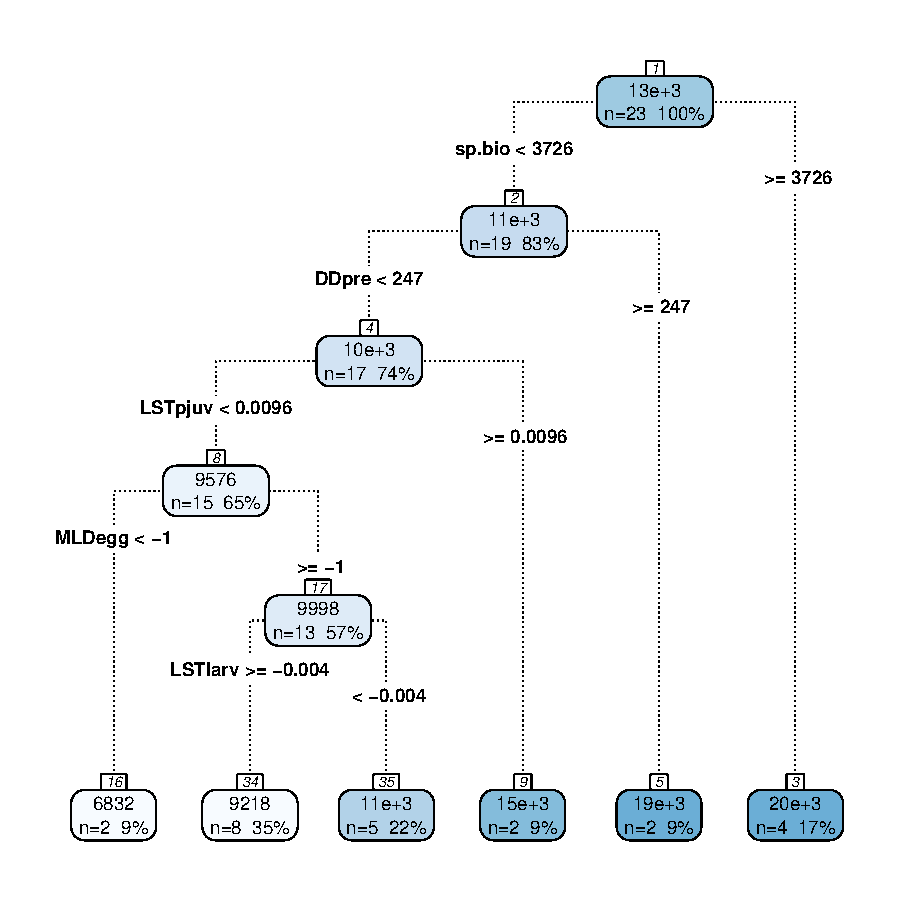
\includegraphics{calcurr_files/figure-latex/unnamed-chunk-4-1.pdf}

\begin{Shaded}
\begin{Highlighting}[]
\KeywordTok{set.seed}\NormalTok{(}\DecValTok{100}\NormalTok{)}
\NormalTok{pet\_split <{-}}\StringTok{ }\KeywordTok{initial\_split}\NormalTok{(wide\_petrale,}\DataTypeTok{prop=}\FloatTok{0.90}\NormalTok{)}
\NormalTok{pet\_train <{-}}\StringTok{ }\KeywordTok{training}\NormalTok{(pet\_split)}

\NormalTok{pet\_recipe <{-}}\StringTok{ }\KeywordTok{recipe}\NormalTok{(age}\FloatTok{.0}\OperatorTok{\textasciitilde{}}\NormalTok{.,}\DataTypeTok{data=}\NormalTok{pet\_train)}

\NormalTok{pet\_prep <{-}}\StringTok{ }\NormalTok{pet\_recipe }\OperatorTok{\%>\%}\StringTok{ }
\StringTok{  }\KeywordTok{prep}\NormalTok{(}\DataTypeTok{training=}\NormalTok{pet\_train,}\DataTypeTok{retain=}\OtherTok{TRUE}\NormalTok{)}

\NormalTok{rf\_model <{-}}\StringTok{ }\KeywordTok{rand\_forest}\NormalTok{(}\DataTypeTok{trees=}\DecValTok{2000}\NormalTok{,}\DataTypeTok{mtry=}\DecValTok{4}\NormalTok{,}\DataTypeTok{mode=}\StringTok{"regression"}\NormalTok{) }\OperatorTok{\%>\%}\StringTok{ }\CommentTok{\#rand\_forest is a function in parsnip.}
\StringTok{  }\KeywordTok{set\_engine}\NormalTok{(}\StringTok{"ranger"}\NormalTok{,}\DataTypeTok{importance=}\StringTok{"permutation"}\NormalTok{) }\OperatorTok{\%>\%}\StringTok{ }\CommentTok{\# rand\_forest is part of the ranger package. We have several options for importance measures.}
\StringTok{  }\KeywordTok{fit}\NormalTok{(age}\FloatTok{.0}\OperatorTok{\textasciitilde{}}\NormalTok{.,}\DataTypeTok{data=}\KeywordTok{juice}\NormalTok{(pet\_prep))}


\CommentTok{\#library(randomForestExplainer)}
\NormalTok{impt\_frame<{-}}\KeywordTok{measure\_importance}\NormalTok{(rf\_model}\OperatorTok{$}\NormalTok{fit)}

\CommentTok{\#impt\_frame \%>\% head()}
\CommentTok{\#  I like this plot as a way to illustate how several of the different RF hyperparameters fall out for different features.}
\KeywordTok{plot\_multi\_way\_importance}\NormalTok{(impt\_frame,}\DataTypeTok{no\_of\_labels =} \DecValTok{6}\NormalTok{)}
\end{Highlighting}
\end{Shaded}

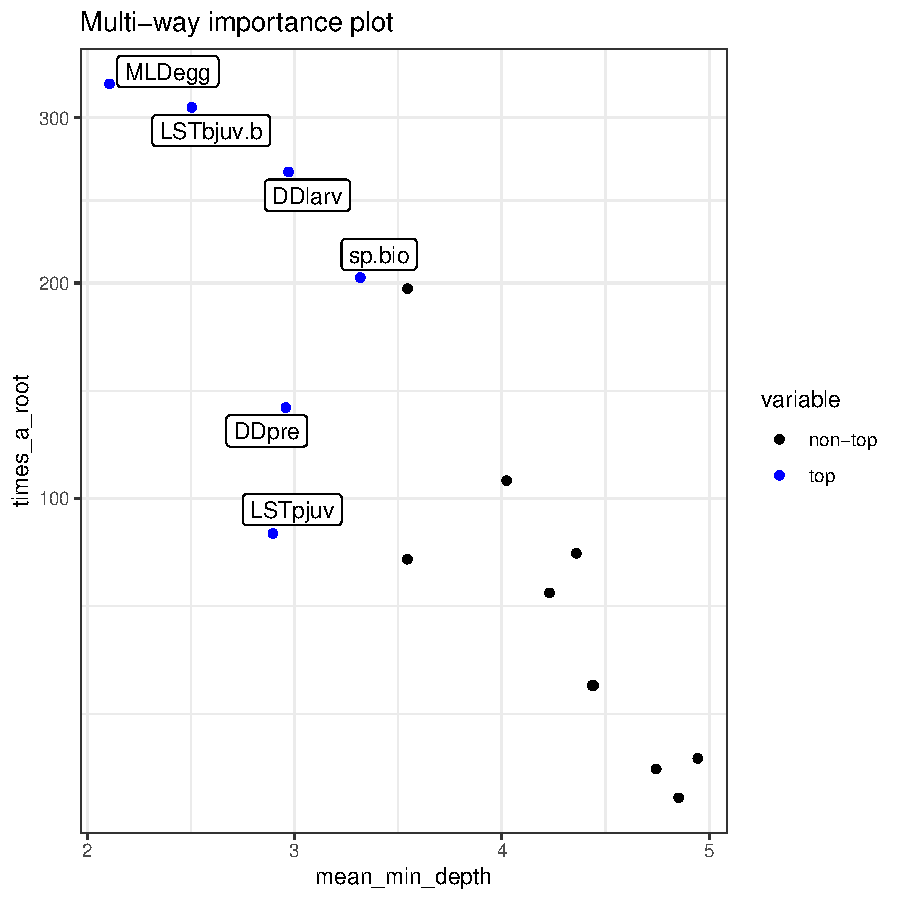
\includegraphics{calcurr_files/figure-latex/unnamed-chunk-4-2.pdf}

So lots of other variables seem to be more important than spawning
biomass.

\begin{Shaded}
\begin{Highlighting}[]
\NormalTok{modpetrale }\OperatorTok{\%>\%}\StringTok{ }
\StringTok{  }\KeywordTok{group\_by}\NormalTok{(name) }\OperatorTok{\%>\%}
\StringTok{  }\KeywordTok{do}\NormalTok{(}\KeywordTok{glance}\NormalTok{(}\KeywordTok{lm}\NormalTok{(age}\FloatTok{.0}\OperatorTok{\textasciitilde{}}\NormalTok{covs\_val,}\DataTypeTok{data=}\NormalTok{.))) }\OperatorTok{\%>\%}
\StringTok{  }\KeywordTok{bind\_rows}\NormalTok{(modpetrale }\OperatorTok{\%>\%}\StringTok{ }
\StringTok{              }\NormalTok{dplyr}\OperatorTok{::}\KeywordTok{select}\NormalTok{(}\OperatorTok{{-}}\KeywordTok{c}\NormalTok{(covs\_val,name)) }\OperatorTok{\%>\%}
\StringTok{              }\KeywordTok{distinct}\NormalTok{() }\OperatorTok{\%>\%}\StringTok{ }
\StringTok{              }\KeywordTok{do}\NormalTok{(}\KeywordTok{glance}\NormalTok{(}\KeywordTok{lm}\NormalTok{(age}\FloatTok{.0}\OperatorTok{\textasciitilde{}}\NormalTok{sp.bio,}\DataTypeTok{data=}\NormalTok{.))) }\OperatorTok{\%>\%}
\StringTok{              }\KeywordTok{mutate}\NormalTok{(}\DataTypeTok{name=}\StringTok{"sp.bio only"}\NormalTok{)) }\OperatorTok{\%>\%}
\StringTok{  }\KeywordTok{arrange}\NormalTok{(}\OperatorTok{{-}}\NormalTok{adj.r.squared) }\OperatorTok{\%>\%}\StringTok{ }
\StringTok{  }\KeywordTok{mutate}\NormalTok{(}\KeywordTok{across}\NormalTok{(}\KeywordTok{where}\NormalTok{(is.double), round, }\DecValTok{3}\NormalTok{)) }\OperatorTok{\%>\%}\StringTok{ }
\StringTok{  }\NormalTok{dplyr}\OperatorTok{::}\KeywordTok{select}\NormalTok{(}\OperatorTok{{-}}\KeywordTok{c}\NormalTok{(r.squared,logLik)) }\OperatorTok{\%>\%}\StringTok{ }
\StringTok{  }\NormalTok{data.frame }\OperatorTok{\%>\%}
\StringTok{  }\KeywordTok{kable}\NormalTok{()}
\end{Highlighting}
\end{Shaded}

\begin{longtable}[]{@{}lrrrrrrrrrr@{}}
\toprule
name & adj.r.squared & sigma & statistic & p.value & df & AIC & BIC &
deviance & df.residual & nobs\tabularnewline
\midrule
\endhead
MLDegg & 0.231 & 4521.897 & 9.713 & 0.004 & 1 & 594.068 & 598.271 &
572531575 & 28 & 30\tabularnewline
LSTbjuv.b & 0.122 & 4832.227 & 5.025 & 0.033 & 1 & 598.050 & 602.254 &
653811791 & 28 & 30\tabularnewline
CSTegg1 & 0.089 & 4922.288 & 3.827 & 0.060 & 1 & 599.158 & 603.362 &
678409764 & 28 & 30\tabularnewline
sp.bio only & 0.047 & 5033.235 & 2.440 & 0.130 & 1 & 600.496 & 604.699 &
709336806 & 28 & 30\tabularnewline
DDpre & 0.042 & 5047.130 & 2.272 & 0.143 & 1 & 600.661 & 604.865 &
713258614 & 28 & 30\tabularnewline
DDpjuv & 0.013 & 5122.238 & 1.391 & 0.248 & 1 & 601.547 & 605.751 &
734645045 & 28 & 30\tabularnewline
Tpre.a & 0.009 & 5134.383 & 1.252 & 0.273 & 1 & 601.689 & 605.893 &
738132917 & 28 & 30\tabularnewline
DDlarv & 0.004 & 5146.356 & 1.116 & 0.300 & 1 & 601.829 & 606.033 &
741579492 & 28 & 30\tabularnewline
LSTegg & -0.004 & 5166.082 & 0.894 & 0.352 & 1 & 602.059 & 606.262 &
747275404 & 28 & 30\tabularnewline
LSTegg2 & -0.009 & 5179.257 & 0.747 & 0.395 & 1 & 602.212 & 606.415 &
751091554 & 28 & 30\tabularnewline
CSTlarv & -0.022 & 5213.963 & 0.366 & 0.550 & 1 & 602.612 & 606.816 &
761191376 & 28 & 30\tabularnewline
CSTpjuv & -0.031 & 5236.641 & 0.121 & 0.731 & 1 & 602.873 & 607.076 &
767827595 & 28 & 30\tabularnewline
LSTlarv & -0.034 & 5242.367 & 0.060 & 0.809 & 1 & 602.938 & 607.142 &
769507417 & 28 & 30\tabularnewline
CSTegg2 & -0.036 & 5247.620 & 0.003 & 0.954 & 1 & 602.998 & 607.202 &
771050514 & 28 & 30\tabularnewline
DDegg1 & -0.036 & 5247.644 & 0.003 & 0.956 & 1 & 602.999 & 607.202 &
771057579 & 28 & 30\tabularnewline
LSTpjuv & -0.036 & 5247.934 & 0.000 & 0.999 & 1 & 603.002 & 607.206 &
771142643 & 28 & 30\tabularnewline
\bottomrule
\end{longtable}

\begin{Shaded}
\begin{Highlighting}[]
\KeywordTok{plot\_importance\_ggpairs}\NormalTok{(impt\_frame)}
\end{Highlighting}
\end{Shaded}

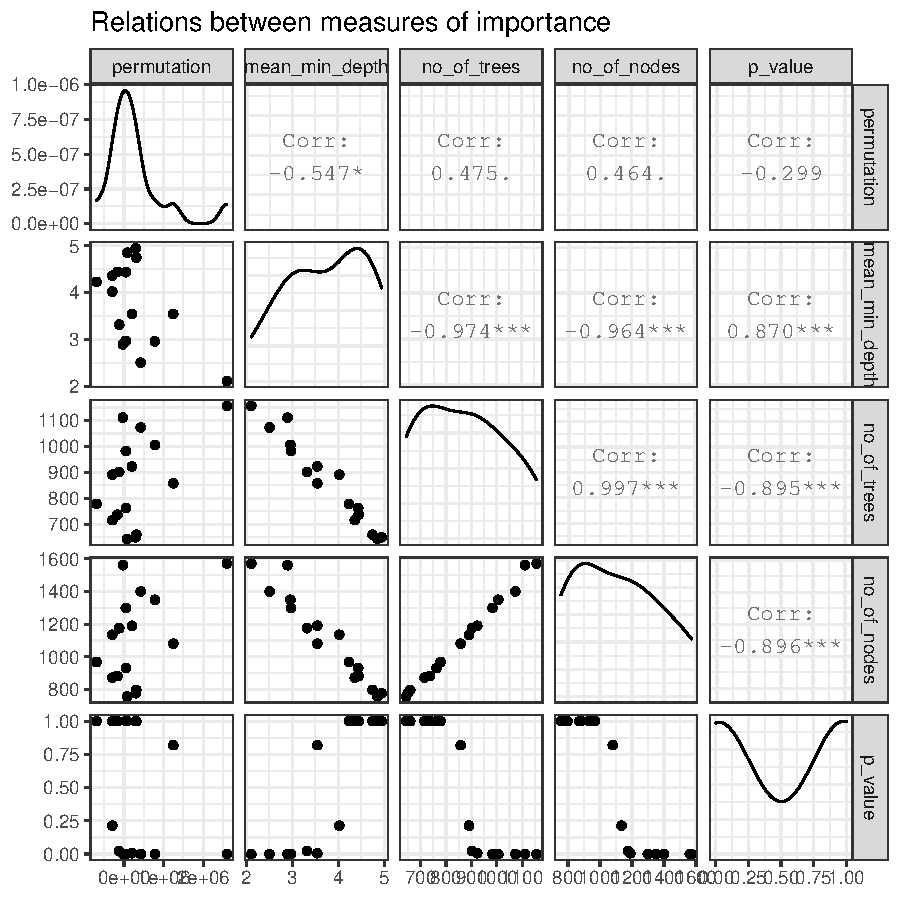
\includegraphics{calcurr_files/figure-latex/unnamed-chunk-6-1.pdf}

\begin{Shaded}
\begin{Highlighting}[]
\NormalTok{md\_frame <{-}}\StringTok{ }\KeywordTok{min\_depth\_distribution}\NormalTok{(rf\_model}\OperatorTok{$}\NormalTok{fit)}

\KeywordTok{plot\_min\_depth\_distribution}\NormalTok{(md\_frame, }\DataTypeTok{mean\_sample =} \StringTok{"top\_trees"}\NormalTok{)}
\end{Highlighting}
\end{Shaded}

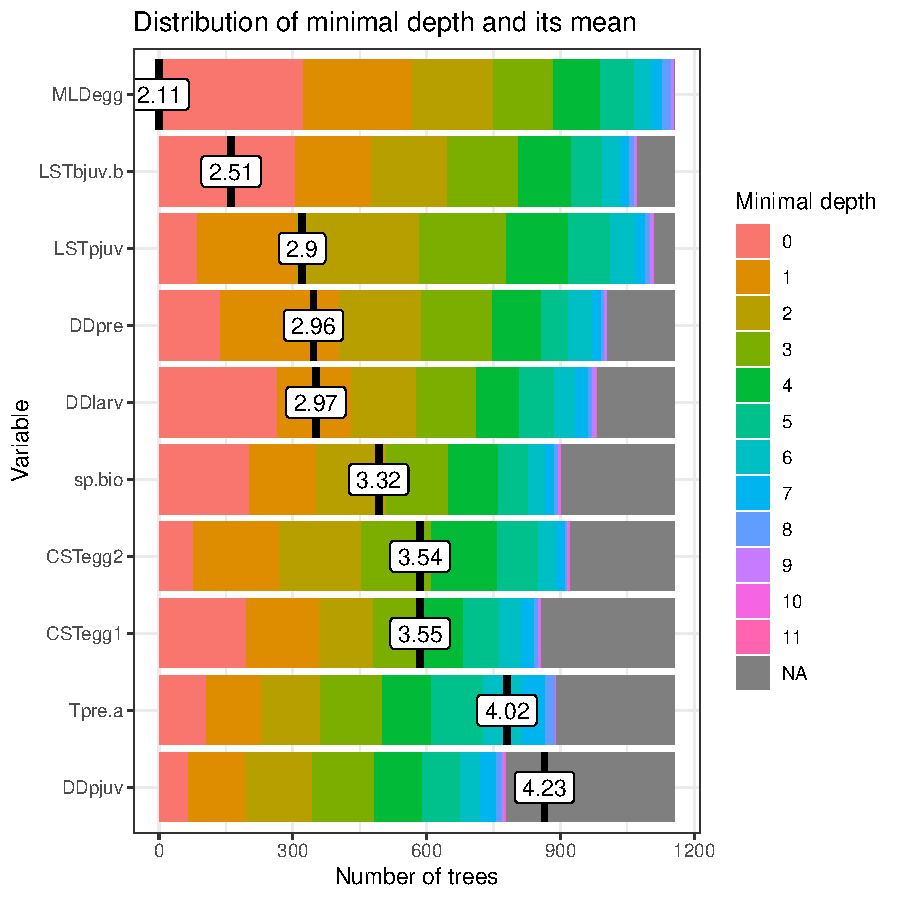
\includegraphics{calcurr_files/figure-latex/unnamed-chunk-7-1.pdf}

\begin{Shaded}
\begin{Highlighting}[]
\KeywordTok{fit\_split}\NormalTok{(age}\FloatTok{.0} \OperatorTok{\textasciitilde{}}\StringTok{ }\NormalTok{., }
          \DataTypeTok{model =} \KeywordTok{rand\_forest}\NormalTok{() }\OperatorTok{\%>\%}\StringTok{ }
\StringTok{            }\KeywordTok{set\_engine}\NormalTok{(}\StringTok{"ranger"}\NormalTok{) }\OperatorTok{\%>\%}\StringTok{ }
\StringTok{            }\KeywordTok{set\_mode}\NormalTok{(}\StringTok{"regression"}\NormalTok{), }
          \DataTypeTok{split =}\NormalTok{ pet\_split) }\OperatorTok{\%>\%}\StringTok{ }
\StringTok{  }\KeywordTok{collect\_metrics}\NormalTok{()}
\end{Highlighting}
\end{Shaded}

\begin{verbatim}
# A tibble: 2 x 3
  .metric .estimator .estimate
  <chr>   <chr>          <dbl>
1 rmse    standard       3793.
2 rsq     standard          1 
\end{verbatim}

Hack the leave one out validation

\begin{Shaded}
\begin{Highlighting}[]
\KeywordTok{initial\_split}\NormalTok{(wide\_petrale, }\DataTypeTok{prop=}\FloatTok{0.96}\NormalTok{)}
\end{Highlighting}
\end{Shaded}

\begin{verbatim}
<Analysis/Assess/Total>
<29/1/30>
\end{verbatim}

\begin{Shaded}
\begin{Highlighting}[]
\KeywordTok{set.seed}\NormalTok{(}\DecValTok{100}\NormalTok{)}
\NormalTok{pet\_split <{-}}\StringTok{ }\KeywordTok{initial\_split}\NormalTok{(wide\_petrale,}\DataTypeTok{prop=}\FloatTok{0.95}\NormalTok{)}
\NormalTok{pet\_train <{-}}\StringTok{ }\KeywordTok{training}\NormalTok{(pet\_split)}
\CommentTok{\#  First specify the model framework}
\NormalTok{tune\_spec <{-}}\StringTok{ }\KeywordTok{rand\_forest}\NormalTok{(}\DataTypeTok{mtry =} \KeywordTok{tune}\NormalTok{(),}
              \DataTypeTok{trees =} \KeywordTok{tune}\NormalTok{(),}
              \DataTypeTok{min\_n =} \KeywordTok{tune}\NormalTok{()) }\OperatorTok{\%>\%}\StringTok{ }
\StringTok{  }\KeywordTok{set\_engine}\NormalTok{(}\StringTok{"ranger"}\NormalTok{) }\OperatorTok{\%>\%}\StringTok{ }
\StringTok{  }\KeywordTok{set\_mode}\NormalTok{(}\StringTok{"regression"}\NormalTok{) }

\CommentTok{\# Now specify the model}
\NormalTok{tune\_wf <{-}}\StringTok{ }\KeywordTok{workflow}\NormalTok{() }\OperatorTok{\%>\%}\StringTok{ }
\StringTok{  }\KeywordTok{add\_recipe}\NormalTok{(pet\_recipe) }\OperatorTok{\%>\%}\StringTok{ }
\StringTok{  }\KeywordTok{add\_model}\NormalTok{(tune\_spec)}
\end{Highlighting}
\end{Shaded}

\begin{Shaded}
\begin{Highlighting}[]
\KeywordTok{dim}\NormalTok{(}\KeywordTok{vfold\_cv}\NormalTok{(wide\_petrale,}\DecValTok{100}\NormalTok{))}
\end{Highlighting}
\end{Shaded}

\begin{verbatim}
[1] 30  2
\end{verbatim}

\begin{Shaded}
\begin{Highlighting}[]
\CommentTok{\#set.seed(234) If you were actually doing random subsets, you\textquotesingle{}d want to set the seed.}
\NormalTok{pet\_folds <{-}}\StringTok{ }\KeywordTok{vfold\_cv}\NormalTok{(pet\_train,}\DecValTok{100}\NormalTok{)}

\CommentTok{\#  Setup parallel processing.}
\NormalTok{cl <{-}}\StringTok{ }\KeywordTok{makeCluster}\NormalTok{(}\DecValTok{3}\NormalTok{)}
\NormalTok{doParallel}\OperatorTok{::}\KeywordTok{registerDoParallel}\NormalTok{(cl)}
\KeywordTok{clusterEvalQ}\NormalTok{(cl, }\KeywordTok{.libPaths}\NormalTok{(}\StringTok{"C:/\textasciitilde{}/R/win{-}library/4.0/"}\NormalTok{))}
\end{Highlighting}
\end{Shaded}

\begin{verbatim}
[[1]]
[1] "C:/~/R/win-library/4.0"             "C:/Program Files/R/R-4.0.1/library"

[[2]]
[1] "C:/~/R/win-library/4.0"             "C:/Program Files/R/R-4.0.1/library"

[[3]]
[1] "C:/~/R/win-library/4.0"             "C:/Program Files/R/R-4.0.1/library"
\end{verbatim}

\begin{Shaded}
\begin{Highlighting}[]
\CommentTok{\#  Now run the model, which is going to try 20 different values for each of the tuning hyperparameters and do this for 10 resamples of the data.}
\KeywordTok{set.seed}\NormalTok{(}\DecValTok{345}\NormalTok{)}
\NormalTok{tune\_res <{-}}\StringTok{ }\KeywordTok{tune\_grid}\NormalTok{(}
\NormalTok{  tune\_wf,}
  \DataTypeTok{resamples =}\NormalTok{ pet\_folds,}
  \DataTypeTok{grid =} \DecValTok{20}
\NormalTok{)}
\end{Highlighting}
\end{Shaded}

\begin{verbatim}
i Creating pre-processing data to finalize unknown parameter: mtry
\end{verbatim}

\begin{Shaded}
\begin{Highlighting}[]
\NormalTok{tune\_res}
\end{Highlighting}
\end{Shaded}

\begin{verbatim}
# Tuning results
# 100-fold cross-validation 
# A tibble: 29 x 4
   splits         id     .metrics          .notes          
   <list>         <chr>  <list>            <list>          
 1 <split [28/1]> Fold01 <tibble [40 x 7]> <tibble [0 x 1]>
 2 <split [28/1]> Fold02 <tibble [40 x 7]> <tibble [0 x 1]>
 3 <split [28/1]> Fold03 <tibble [40 x 7]> <tibble [0 x 1]>
 4 <split [28/1]> Fold04 <tibble [40 x 7]> <tibble [0 x 1]>
 5 <split [28/1]> Fold05 <tibble [40 x 7]> <tibble [0 x 1]>
 6 <split [28/1]> Fold06 <tibble [40 x 7]> <tibble [0 x 1]>
 7 <split [28/1]> Fold07 <tibble [40 x 7]> <tibble [0 x 1]>
 8 <split [28/1]> Fold08 <tibble [40 x 7]> <tibble [0 x 1]>
 9 <split [28/1]> Fold09 <tibble [40 x 7]> <tibble [0 x 1]>
10 <split [28/1]> Fold10 <tibble [40 x 7]> <tibble [0 x 1]>
# ... with 19 more rows
\end{verbatim}

\begin{Shaded}
\begin{Highlighting}[]
\NormalTok{tune\_res }\OperatorTok{\%>\%}
\StringTok{  }\KeywordTok{collect\_metrics}\NormalTok{() }\OperatorTok{\%>\%}\StringTok{ }
\StringTok{  }\KeywordTok{filter}\NormalTok{(.metric}\OperatorTok{==}\StringTok{"rmse"}\NormalTok{) }\OperatorTok{\%>\%}\StringTok{ }
\StringTok{  }\KeywordTok{arrange}\NormalTok{(mean)}
\end{Highlighting}
\end{Shaded}

\begin{verbatim}
# A tibble: 20 x 9
    mtry trees min_n .metric .estimator  mean     n std_err .config
   <int> <int> <int> <chr>   <chr>      <dbl> <int>   <dbl> <chr>  
 1    12   453    32 rmse    standard   3943.    29    669. Model04
 2    15   569    30 rmse    standard   3946.    29    671. Model07
 3    11    70    27 rmse    standard   3954.    29    653. Model16
 4    14  1234    38 rmse    standard   3955.    29    668. Model20
 5    14   935    37 rmse    standard   3959.    29    669. Model15
 6     9   162    33 rmse    standard   3960.    29    665. Model03
 7    11  1437    35 rmse    standard   3969.    29    668. Model18
 8     6   299    25 rmse    standard   3998.    29    640. Model06
 9     7  1680     8 rmse    standard   4029.    29    625. Model12
10     5   687     5 rmse    standard   4033.    29    618. Model17
11     3  1365     9 rmse    standard   4033.    29    608. Model14
12     5   803    14 rmse    standard   4035.    29    625. Model19
13     1   788     3 rmse    standard   4040.    29    618. Model13
14     2  1911    18 rmse    standard   4042.    29    621. Model08
15     3  1101    20 rmse    standard   4050.    29    613. Model05
16     9   306    23 rmse    standard   4059.    29    657. Model10
17     7  1581    10 rmse    standard   4061.    29    628. Model02
18     8  1099    12 rmse    standard   4077.    29    629. Model11
19    15  1776    26 rmse    standard   4121.    29    658. Model09
20    12  1831    17 rmse    standard   4150.    29    643. Model01
\end{verbatim}

\begin{Shaded}
\begin{Highlighting}[]
\NormalTok{tune\_res }\OperatorTok{\%>\%}
\StringTok{  }\KeywordTok{collect\_metrics}\NormalTok{() }\OperatorTok{\%>\%}
\StringTok{  }\KeywordTok{filter}\NormalTok{(.metric }\OperatorTok{==}\StringTok{ "rmse"}\NormalTok{) }\OperatorTok{\%>\%}
\StringTok{  }\KeywordTok{select}\NormalTok{(mean, min\_n, mtry, trees) }\OperatorTok{\%>\%}
\StringTok{  }\KeywordTok{pivot\_longer}\NormalTok{(}\KeywordTok{c}\NormalTok{(min\_n,mtry,trees),}
    \DataTypeTok{values\_to =} \StringTok{"value"}\NormalTok{,}
    \DataTypeTok{names\_to =} \StringTok{"parameter"}
\NormalTok{  ) }\OperatorTok{\%>\%}
\StringTok{  }\KeywordTok{ggplot}\NormalTok{(}\KeywordTok{aes}\NormalTok{(value, mean, }\DataTypeTok{color =}\NormalTok{ parameter)) }\OperatorTok{+}
\StringTok{  }\KeywordTok{geom\_point}\NormalTok{(}\DataTypeTok{show.legend =} \OtherTok{FALSE}\NormalTok{) }\OperatorTok{+}
\StringTok{  }\KeywordTok{facet\_wrap}\NormalTok{(}\OperatorTok{\textasciitilde{}}\NormalTok{parameter, }\DataTypeTok{scales =} \StringTok{"free\_x"}\NormalTok{) }\OperatorTok{+}
\StringTok{  }\KeywordTok{labs}\NormalTok{(}\DataTypeTok{x =} \OtherTok{NULL}\NormalTok{, }\DataTypeTok{y =} \StringTok{"rmse"}\NormalTok{)}
\end{Highlighting}
\end{Shaded}

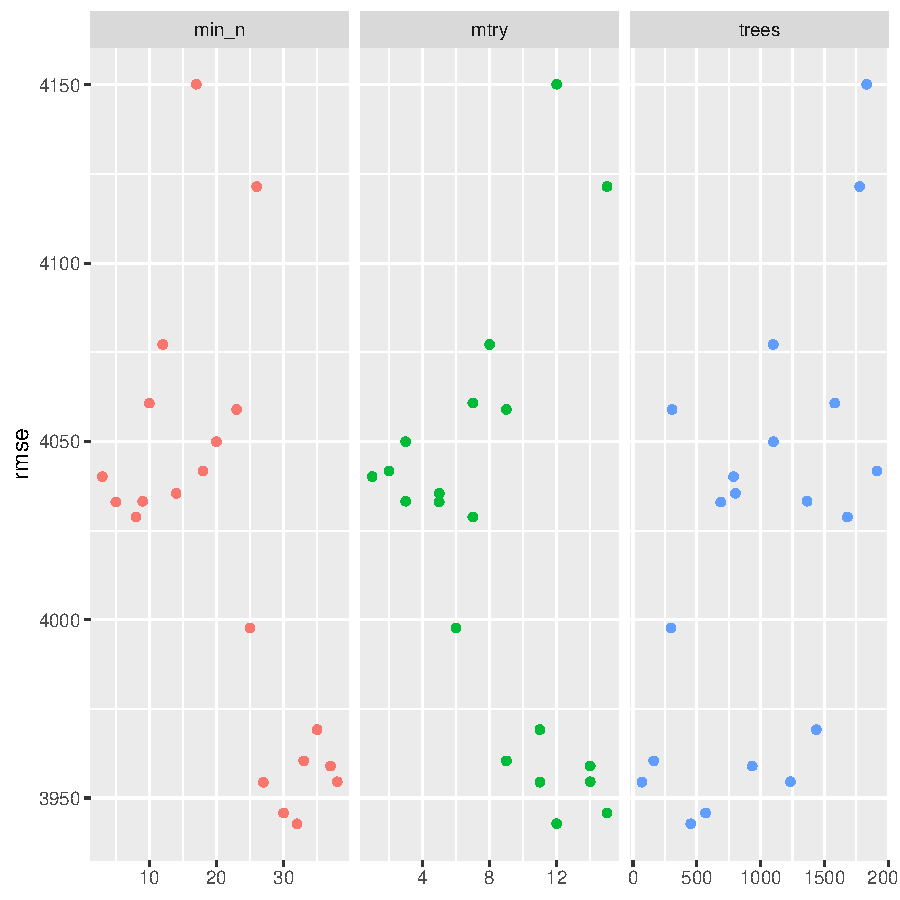
\includegraphics{calcurr_files/figure-latex/unnamed-chunk-13-1.pdf}

\begin{Shaded}
\begin{Highlighting}[]
\NormalTok{best\_rmse <{-}}\StringTok{ }\KeywordTok{select\_best}\NormalTok{(tune\_res,}\StringTok{"rmse"}\NormalTok{)}

\NormalTok{best\_rmse}
\end{Highlighting}
\end{Shaded}

\begin{verbatim}
# A tibble: 1 x 4
   mtry trees min_n .config
  <int> <int> <int> <chr>  
1    12   453    32 Model04
\end{verbatim}

\begin{Shaded}
\begin{Highlighting}[]
\NormalTok{final\_rf <{-}}\StringTok{ }\KeywordTok{finalize\_model}\NormalTok{(}
\NormalTok{  tune\_spec,}
\NormalTok{  best\_rmse}
\NormalTok{)}

\NormalTok{final\_rf }\OperatorTok{\%>\%}
\StringTok{  }\KeywordTok{set\_engine}\NormalTok{(}\StringTok{"ranger"}\NormalTok{, }\DataTypeTok{importance =} \StringTok{"permutation"}\NormalTok{) }\OperatorTok{\%>\%}
\StringTok{  }\KeywordTok{fit}\NormalTok{(age}\FloatTok{.0} \OperatorTok{\textasciitilde{}}\StringTok{ }\NormalTok{.,}
    \DataTypeTok{data =} \KeywordTok{juice}\NormalTok{(pet\_prep)) }\OperatorTok{\%>\%}
\StringTok{  }\NormalTok{vip}\OperatorTok{::}\KeywordTok{vip}\NormalTok{(}\DataTypeTok{geom =} \StringTok{"point"}\NormalTok{)}
\end{Highlighting}
\end{Shaded}

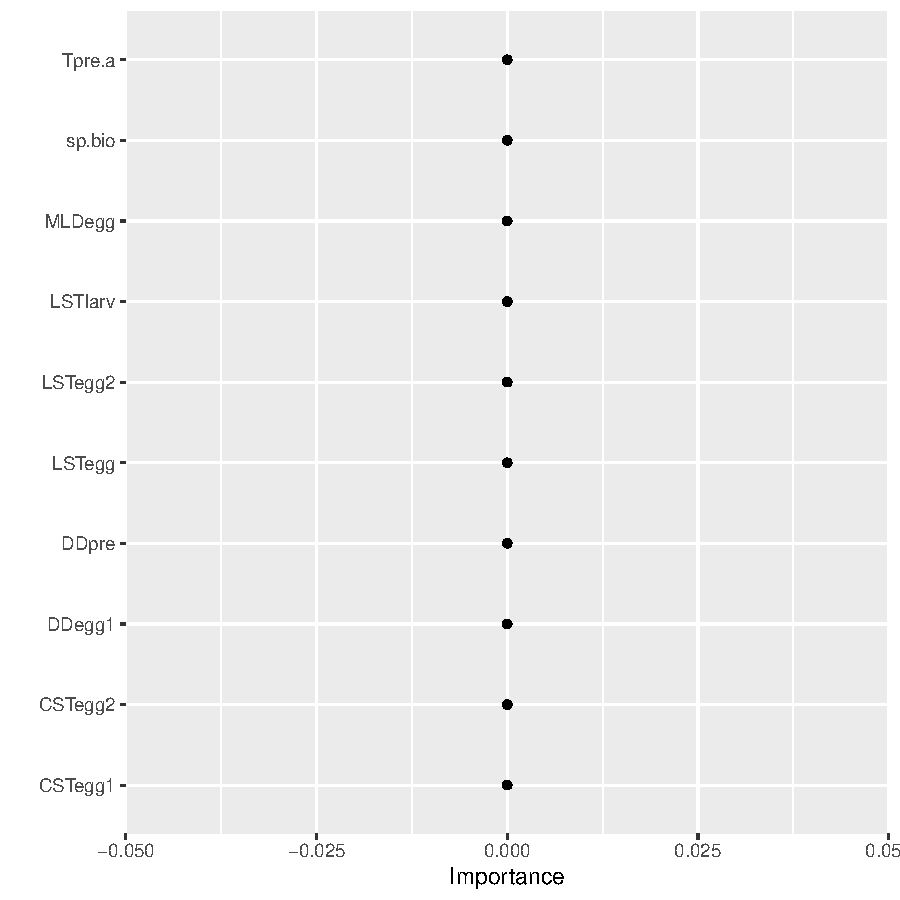
\includegraphics{calcurr_files/figure-latex/unnamed-chunk-14-1.pdf}

\begin{Shaded}
\begin{Highlighting}[]
\KeywordTok{rand\_forest}\NormalTok{(}\DataTypeTok{trees=}\DecValTok{1911}\NormalTok{,}\DataTypeTok{mtry=}\DecValTok{7}\NormalTok{,}\DataTypeTok{min\_n=}\DecValTok{18}\NormalTok{,}\DataTypeTok{mode=}\StringTok{"regression"}\NormalTok{) }\OperatorTok{\%>\%}\StringTok{ }\CommentTok{\#rand\_forest is a function in parsnip.}
\StringTok{  }\KeywordTok{set\_engine}\NormalTok{(}\StringTok{"ranger"}\NormalTok{,}\DataTypeTok{importance=}\StringTok{"permutation"}\NormalTok{) }\OperatorTok{\%>\%}\StringTok{ }\CommentTok{\# rand\_forest is part of the ranger package. We have several options for importance measures.}
\StringTok{  }\KeywordTok{fit}\NormalTok{(age}\FloatTok{.0}\OperatorTok{\textasciitilde{}}\NormalTok{.,}\DataTypeTok{data=}\KeywordTok{juice}\NormalTok{(pet\_prep)) }\OperatorTok{\%>\%}\StringTok{ }
\StringTok{  }\KeywordTok{vip}\NormalTok{()}
\end{Highlighting}
\end{Shaded}

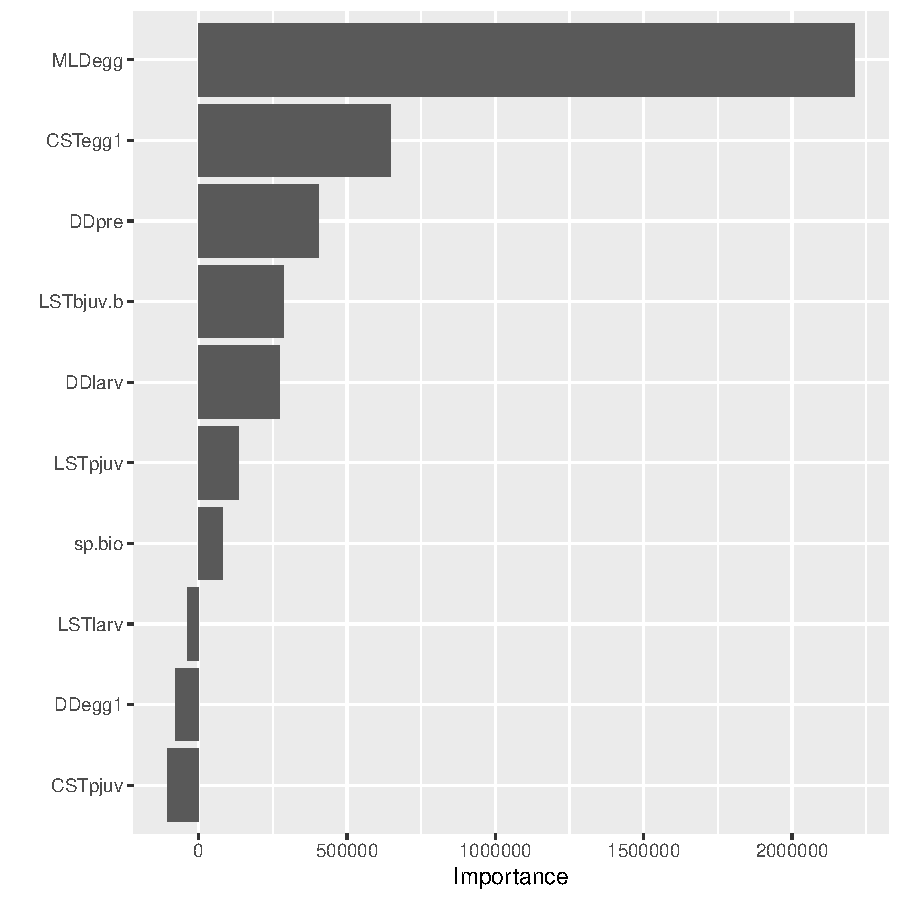
\includegraphics{calcurr_files/figure-latex/unnamed-chunk-14-2.pdf}

\begin{Shaded}
\begin{Highlighting}[]
\NormalTok{final\_rf }\OperatorTok{\%>\%}
\StringTok{  }\KeywordTok{set\_engine}\NormalTok{(}\StringTok{"ranger"}\NormalTok{, }\DataTypeTok{importance =} \StringTok{"impurity"}\NormalTok{) }\OperatorTok{\%>\%}
\StringTok{  }\KeywordTok{fit}\NormalTok{(age}\FloatTok{.0} \OperatorTok{\textasciitilde{}}\StringTok{ }\NormalTok{.,}
    \DataTypeTok{data =} \KeywordTok{juice}\NormalTok{(pet\_prep)) }\OperatorTok{\%>\%}
\StringTok{  }\NormalTok{vip}\OperatorTok{::}\KeywordTok{vip}\NormalTok{(}\DataTypeTok{geom =} \StringTok{"point"}\NormalTok{)}
\end{Highlighting}
\end{Shaded}

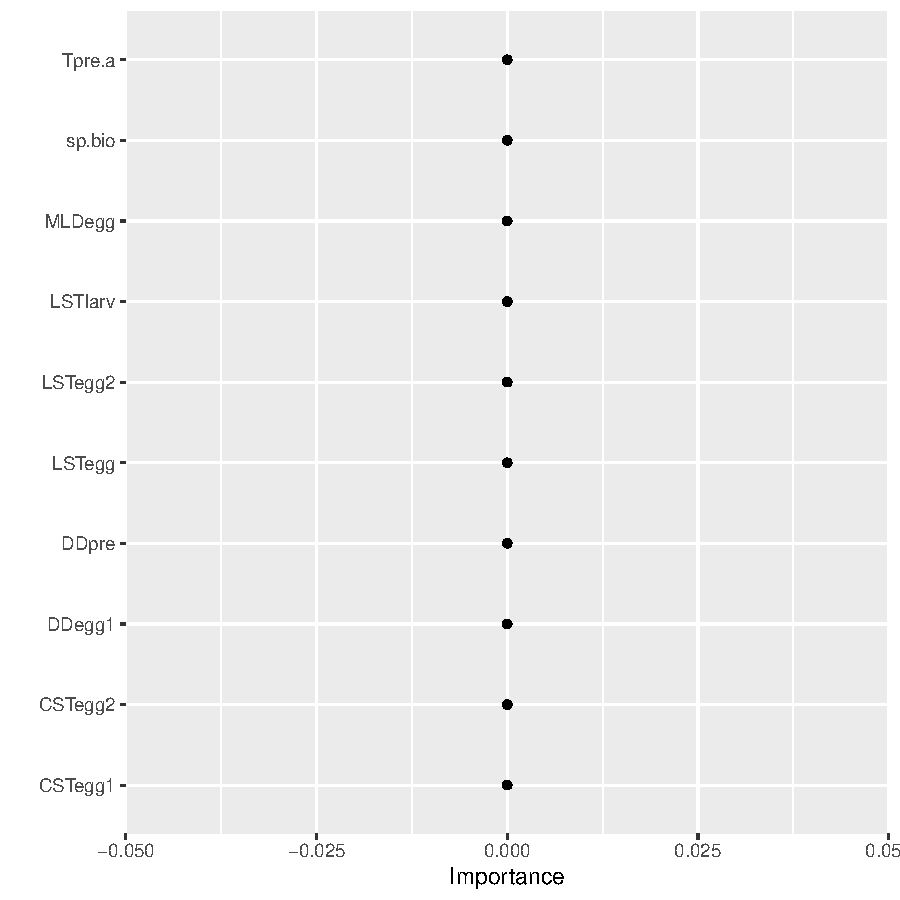
\includegraphics{calcurr_files/figure-latex/unnamed-chunk-14-3.pdf}

\end{document}
